\documentclass[10pt,twocolumn]{article}
\usepackage{geometry}
\usepackage[utf8]{inputenc}
\usepackage[spanish]{babel}
\usepackage{amsmath} 
\usepackage{cases}
\usepackage{graphicx}

\geometry{margin=0.8in}

\graphicspath{{./figs/}}

\begin{document}

\author{Nahuel Almeira}

\title{Redes Neuronales 2020\\ FaMAF, UNC\\ Práctico 2}

\maketitle

\section{Introducción}

En este práctico trabajaremos con una red neuronal de tipo \emph{autoencoder} sobre el conjunto de datos MNIST.

Un autoencoder es un tipo de red neuronal \emph{feed-forward}, cuyo objetivo es aprender la función identidad sobre un conjunto de datos. Una manera de representar esta red es la siguiente. Supongamos que contamos con un dataset $X\in \mathcal{R}^n$, cuyos elementos, llamados datos puntuales, denominamos como $x$. Un autoencoder cuenta con dos etapas. Una etapa de codificación, o \emph{encoder}, donde se aplica una función $f$ sobre los datos para producir el código $h = f(x)$. Luego, este código es decodificado en la segunda parte del autoencoder, denominada \emph{decoder}, mediante una función $g$, tal que $\hat{x} = g(h) = g(f(x))$. En general, la salida de la red no coincide exactamente con el dato ingresado, sino que es una versión ligeramente distinta del mismo. La idea del autoencoder es aprender la función identidad de manera aproximada, y no de forma exacta.

Entre las aplicaciones que pueden tener los autoencoder mencionaremos dos. La primera tiene que ver con el código $h$. Si la dimensión de $h$ es menor que la dimensión de $x$, entonces la red es capaz de reducir la dimensionalidad de los datos sin perder demasiada información. En este caso, no es la salida de la red lo que nos interesa, sino más bien el código en sí. 

La segunda aplicación son los autoencoders con corrección de ruido. En este caso, se busca que, al recibir una entrada $\tilde{x}$ correspondiente a una versión ligeramente corrupta o modificada de $x$, el autoencoder sea capaz de revertir el cambio y devolver una versión corregida, más cercana al dato original.

El desempeño del autoencoder se puede medir con diferentes funciones de costo. En este práctico emplearemos el error cuadrático medio (MSE) definido como

\begin{equation}
L(\hat{x}, x) = \dfrac{1}{n} \sum_{i=1}^n (\hat{x}_i - x_i)^2.
\end{equation}

\section{Dataset}

El dataset MNIST \cite{LeCun} consiste imágenes de dígitos escritos a mano, recolectados por el Instituto Nacional de Estándares y Tecnología de Estados Unidos (NIST, por sus siglas en inglés). Las imágenes tienen un tamaño de $28\times28$ pixeles en escala de grises con 256 valores de intensidad. Además, han sido preprocesadas de manera tal de que los números se ubiquen relativamente centrados y verticales. Cada imagen cuenta a su vez con una etiqueta, que informa el dígito correspondiente. 

En la figura \ref{fig:ejemplos} se pueden ver algunos de los elementos del dataset.


\begin{figure}[th]
\centering
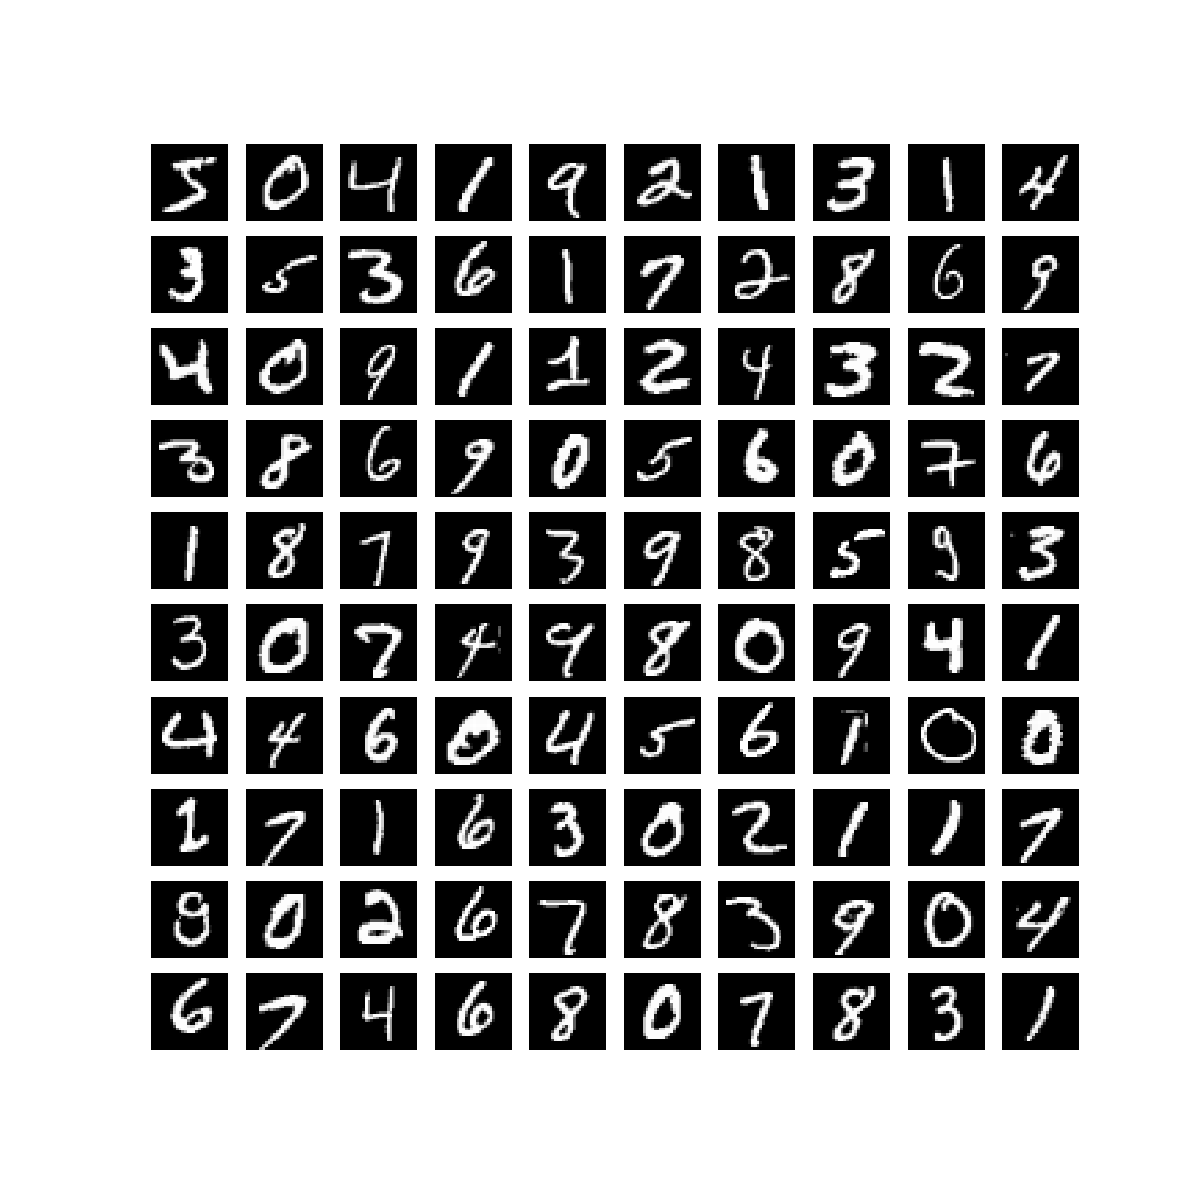
\includegraphics[scale=0.45]{ejemplos.pdf}
\caption{\label{fig:ejemplos} Algunos ejemplos del dataset MNIST.}
\end{figure}

El dataset está dividido en un conjunto de entrenamiento de $60000$ imágenes, y un conjunto de evaluación de $10000$. 



\begin{thebibliography}{9}
\bibitem{LeCun} 
Y. LeCun, L. Bottou, Y. Bengio, and P. Haffner. "Gradient-based learning applied to document recognition." Proceedings of the IEEE, 86(11):2278-2324, November 1998.
\end{thebibliography}

\end{document}
